\section{Date: 2026-10-25}
\noindent \textbf{Series ID: WUIMAYEM} 

\noindent This series is titled Smoothed World Uncertainty Index for Yemen and has a frequency of Quarterly. The units are Index and the seasonal adjustment is Not Seasonally Adjusted.The observation start date is 1971-07-01 and the observation end date is 2026-07-01.The popularity of this series is 1. \\ 

\noindent \textbf{Series ID: IM58} 

\noindent This series is titled Import Price Index (SITC): Plastics in nonprimary forms (DISCONTINUED) and has a frequency of Monthly. The units are Index 2000=100 and the seasonal adjustment is Not Seasonally Adjusted.The observation start date is 1995-01-01 and the observation end date is 2005-12-01.The popularity of this series is 1. \\ 

\subsection{Raw Regression}
\noindent Regresses the two series against each other directly. A significant result here can come just as easily from both series sharing a long-run trend as from any real relationship.

\begin{center}
\begin{tabular}{lclc}
\toprule
\textbf{Dep. Variable:}        & value\_fred\_IM58 & \textbf{  R-squared:         } &     0.033   \\
\textbf{Model:}                &        OLS        & \textbf{  Adj. R-squared:    } &     0.009   \\
\textbf{Method:}               &   Least Squares   & \textbf{  F-statistic:       } &     1.412   \\
\textbf{Date:}                 &  Sun, 25 Oct 2026 & \textbf{  Prob (F-statistic):} &    0.241    \\
\textbf{Time:}                 &      15:07:30     & \textbf{  Log-Likelihood:    } &   -154.05   \\
\textbf{No. Observations:}     &           44      & \textbf{  AIC:               } &     312.1   \\
\textbf{Df Residuals:}         &           42      & \textbf{  BIC:               } &     315.7   \\
\textbf{Df Model:}             &            1      & \textbf{                     } &             \\
\textbf{Covariance Type:}      &     nonrobust     & \textbf{                     } &             \\
\bottomrule
\end{tabular}
\begin{tabular}{lcccccc}
                               & \textbf{coef} & \textbf{std err} & \textbf{t} & \textbf{P$> |$t$|$} & \textbf{[0.025} & \textbf{0.975]}  \\
\midrule
\textbf{const}                 &     105.9204  &        1.811     &    58.494  &         0.000        &      102.266    &      109.575     \\
\textbf{value\_fred\_WUIMAYEM} &     -69.8045  &       58.742     &    -1.188  &         0.241        &     -188.351    &       48.742     \\
\bottomrule
\end{tabular}
\begin{tabular}{lclc}
\textbf{Omnibus:}       & 17.535 & \textbf{  Durbin-Watson:     } &    0.168  \\
\textbf{Prob(Omnibus):} &  0.000 & \textbf{  Jarque-Bera (JB):  } &   22.165  \\
\textbf{Skew:}          &  1.336 & \textbf{  Prob(JB):          } & 1.54e-05  \\
\textbf{Kurtosis:}      &  5.224 & \textbf{  Cond. No.          } &     47.5  \\
\bottomrule
\end{tabular}
%\caption{OLS Regression Results}
\end{center}

Notes: \newline
 [1] Standard Errors assume that the covariance matrix of the errors is correctly specified.

\begin{figure}
\centering
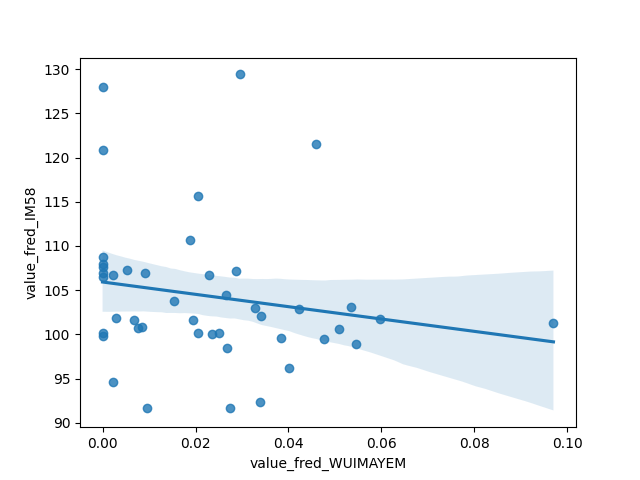
\includegraphics[scale = 0.9]{plots/plot_2026-10-25.png}
\caption{Raw Regression Plot for 2026-10-25}
\end{figure}
\newpage
\subsection{Detrended Regression}
\noindent Regresses the residuals of each series after removing its own linear time trend, so a shared trend can no longer drive the result on its own. A relationship that stays significant here is better evidence of a genuine link between the two series.

\begin{center}
\begin{tabular}{lclc}
\toprule
\textbf{Dep. Variable:}                   & value\_fred\_IM58\_detrended & \textbf{  R-squared:         } &     0.008   \\
\textbf{Model:}                           &             OLS              & \textbf{  Adj. R-squared:    } &    -0.016   \\
\textbf{Method:}                          &        Least Squares         & \textbf{  F-statistic:       } &    0.3384   \\
\textbf{Date:}                            &       Sun, 25 Oct 2026       & \textbf{  Prob (F-statistic):} &    0.564    \\
\textbf{Time:}                            &           15:07:30           & \textbf{  Log-Likelihood:    } &   -149.65   \\
\textbf{No. Observations:}                &                44            & \textbf{  AIC:               } &     303.3   \\
\textbf{Df Residuals:}                    &                42            & \textbf{  BIC:               } &     306.9   \\
\textbf{Df Model:}                        &                 1            & \textbf{                     } &             \\
\textbf{Covariance Type:}                 &          nonrobust           & \textbf{                     } &             \\
\bottomrule
\end{tabular}
\begin{tabular}{lcccccc}
                                          & \textbf{coef} & \textbf{std err} & \textbf{t} & \textbf{P$> |$t$|$} & \textbf{[0.025} & \textbf{0.975]}  \\
\midrule
\textbf{const}                            &   -2.291e-12  &        1.120     & -2.05e-12  &         1.000        &       -2.260    &        2.260     \\
\textbf{value\_fred\_WUIMAYEM\_detrended} &     -31.7583  &       54.595     &    -0.582  &         0.564        &     -141.935    &       78.418     \\
\bottomrule
\end{tabular}
\begin{tabular}{lclc}
\textbf{Omnibus:}       &  2.933 & \textbf{  Durbin-Watson:     } &    0.171  \\
\textbf{Prob(Omnibus):} &  0.231 & \textbf{  Jarque-Bera (JB):  } &    1.845  \\
\textbf{Skew:}          &  0.398 & \textbf{  Prob(JB):          } &    0.398  \\
\textbf{Kurtosis:}      &  3.612 & \textbf{  Cond. No.          } &     48.7  \\
\bottomrule
\end{tabular}
%\caption{OLS Regression Results}
\end{center}

Notes: \newline
 [1] Standard Errors assume that the covariance matrix of the errors is correctly specified.

\begin{figure}
\centering
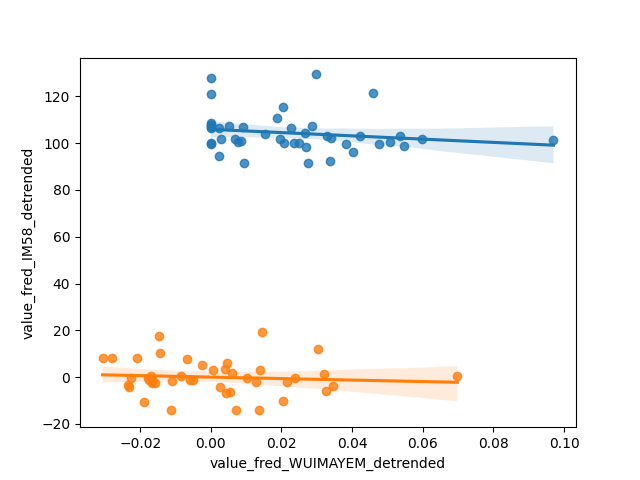
\includegraphics[scale = 0.9]{plots/plot_2026-10-25_detrended.png}
\caption{Detrended Regression Plot for 2026-10-25}
\end{figure}
\newpage
